\section{Threshold-Sensitivity Sweep}\label{sec:extreme_sensitivity}

\textbf{Research question:}

\begin{quote}
Which candidate percentile / persistence-duration configurations for the extreme-weather
definition (Section~\ref{sec:extreme_def}) provide an adequate number of extreme and normal-reference samples that follow the frequency of extreme weather events?
\end{quote}

\subsection{Data and Method}

Before committing to one threshold choice, we swept a grid of candidate configurations---every
combination of percentile pair (90/10, 95/5, 99/1) and persistence duration
($D \in \{4,8,12,16,20,24\}$ hours)---and, for each of the 18 cells, counted four raw quantities
summed across all five variable/technology combinations defined in Section~\ref{sec:extreme_def}
($k_t$, Temperature\_C, and WindSpeed\_mps for the \num{896} solar sites; Temperature\_C and
WindSpeed\_100m\_mps for the \num{114} wind sites): extreme hours, extreme events, normal-reference
hours, and normal-reference events. The sweep sums across all five extreme-variable classifications
($k_t$, Temperature\_C, and WindSpeed\_mps for solar sites and Temperature\_C and WindSpeed\_100m\_mps for wind sites)
over the \num{1010} sites and the 30-year baseline, in terms of hours are number of events.
Raw counts are converted to two derived views: hours as a percentage of the variable's own monitored hours, and events per site per year
(raw events divided by $\num{1010}\times\num{30}$ site-years).

\subsection{Results from the sweep}

Figures~\ref{fig:events_per_site_heatmap} and~\ref{fig:normal_events_per_site_heatmap} visualize the number of extreme and normal weather events, respectively, on average per year and per site depending on the threshold pairing.

\begin{figure}[H]
  \centering
  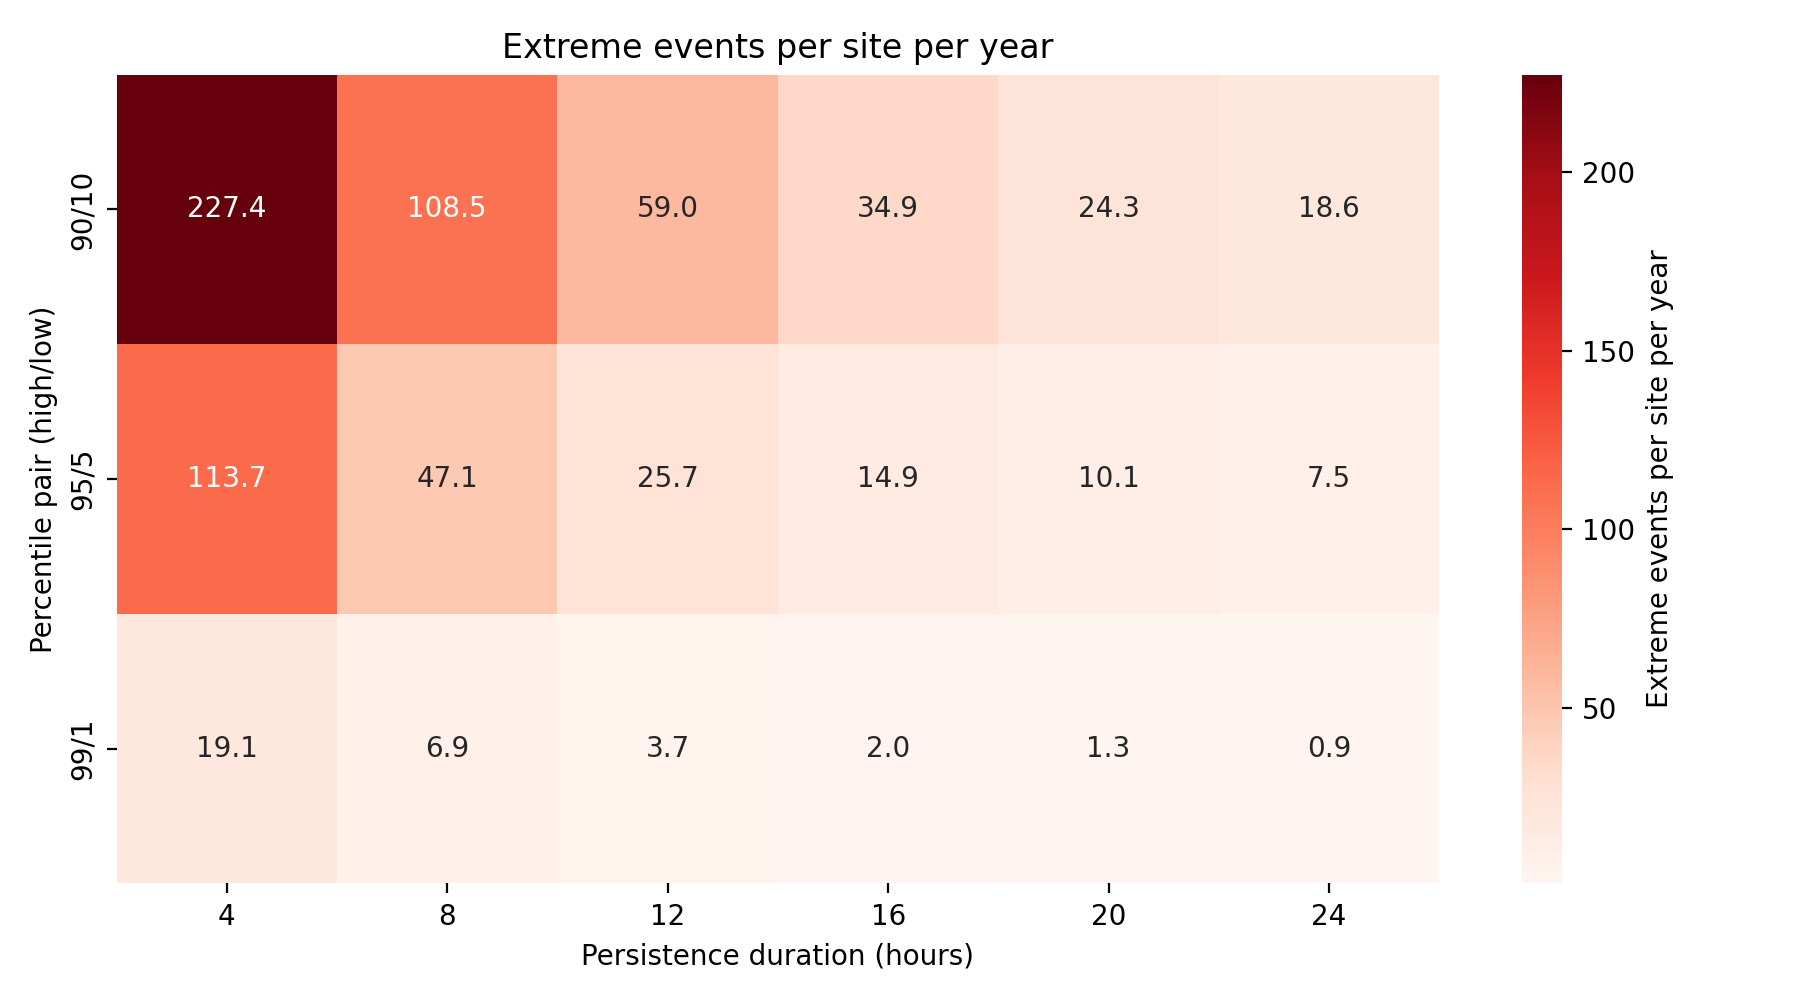
\includegraphics[width=0.8\textwidth]{figures/Q10_extreme_weather/era5_threshold_sensitivity_events_per_site_heatmap.png}
  \caption{Extreme events per site per year. At the loosest cell (90/10, $D=4$\,h) a typical site
  registers $\approx$227 extreme events per year across the five variable/technology combinations;
  at the strictest cell (99/1, $D=24$\,h) this falls to $\approx$0.9---consistent with the
  hour-count collapse in Figure~\ref{fig:extreme_hours_heatmap}, now expressed as a rate a grid
  operator can sanity-check directly (i.e., ``about one extreme, day-long event per site per
  year'').}
  \label{fig:events_per_site_heatmap}
\end{figure}

\begin{figure}[H]
  \centering
  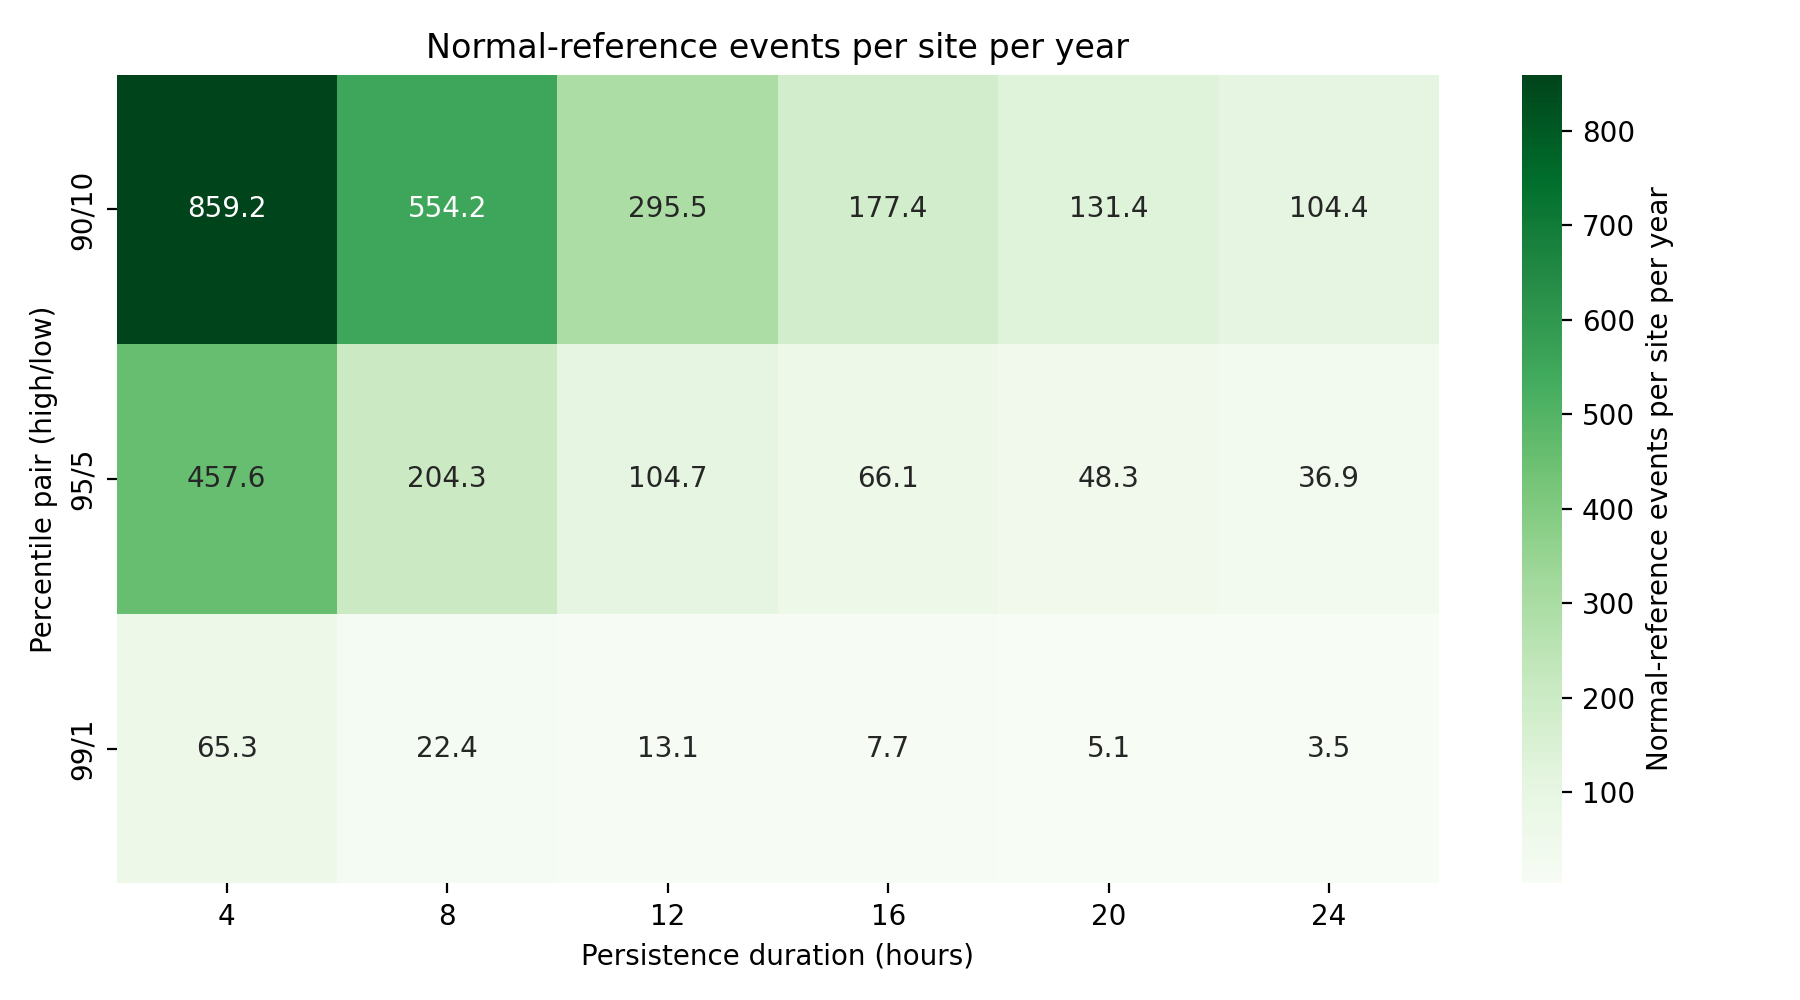
\includegraphics[width=0.8\textwidth]{figures/Q10_extreme_weather/era5_threshold_sensitivity_normal_events_per_site_heatmap.png}
  \caption{Normal-reference events per site per year. Because each qualifying extreme event
  contributes up to two $\pm$5-day matched-control windows (one at each boundary), the
  normal-reference event rate tracks the extreme event rate closely.}
  \label{fig:normal_events_per_site_heatmap}
\end{figure}

Table~\ref{tab:hours_pct} reports the same extreme- and normal-reference-hour results as a
percentage of each configuration's own monitored-hour total, which is the form used to judge
sample-size adequacy directly.

\begin{table}[H]
\centering
\begin{threeparttable}
\caption{Extreme-hours and normal-reference-hours as a percentage of monitored hours, by
percentile pair and persistence duration $D$ (hours).}
\label{tab:hours_pct}
\begin{tabular}{lcccccc}
\toprule
\textbf{Percentile pair} & \textbf{$D{=}4$} & \textbf{$D{=}8$} & \textbf{$D{=}12$} & \textbf{$D{=}16$} & \textbf{$D{=}20$} & \textbf{$D{=}24$} \\
\midrule
\multicolumn{7}{l}{\textit{Extreme hours (\%)}} \\
90/10 & \num{11.601} & \num{8.707}  & \num{6.575} & \num{5.091} & \num{4.239} & \num{3.663} \\
95/5  & \num{5.196}  & \num{3.596}  & \num{2.677} & \num{2.015} & \num{1.628} & \num{1.367} \\
99/1  & \num{0.768}  & \num{0.479}  & \num{0.340} & \num{0.235} & \num{0.177} & \num{0.139} \\
\addlinespace
\multicolumn{7}{l}{\textit{Normal-reference hours (\%)}} \\
90/10 & \num{69.121} & \num{48.834} & \num{31.913} & \num{21.955} & \num{16.742} & \num{13.497} \\
95/5  & \num{56.182} & \num{29.775} & \num{18.291} & \num{11.815} & \num{8.592}  & \num{6.572} \\
99/1  & \num{14.851} & \num{5.996}  & \num{3.418}  & \num{1.924}  & \num{1.250}  & \num{0.879} \\
\bottomrule
\end{tabular}
\begin{tablenotes}
\scriptsize
    \item \textit{Note:} Percentages are of each variable's own monitored-hour total, summed
    across all five variable/technology combinations and \num{1010} sites over the 30-year
    baseline (\num{648053822} monitored variable-hours). Even at the strictest tested cell
    (99/1, $D=24$), both classes remain well above zero (\num{0.139}\% extreme,
    \num{0.879}\% normal-reference), so sample size is not a bottleneck at any tested
    configuration.
\end{tablenotes}
\end{threeparttable}
\end{table}

\subsection{Parameter selection}\label{sec:param_selection}

We select the \textbf{99th/1st percentile pair with an 8-hour persistence duration} as the
operative extreme-weather definition. Table~\ref{tab:hours_pct} shows that sample size is
comfortable even at the strictest tested percentile pair, so there is no need to trade threshold
purity for sample count---the 99/1 pair can be used at its full strictness, isolating genuinely
rare conditions rather than the top decile used as the conventional default in the heat-wave
literature \citep{perkinsalexander2013}. Among the six tested durations, 8 hours balances a
persistence requirement long enough to represent a genuine sustained regime (a heat build-up, a
wind lull, a multi-hour cloud deck) against giving grid operators a realistically actionable
reaction window, and keeps the resulting event rate in the range expected for a genuinely rare
condition---a handful of events per site per year, not one every few days.

At this configuration (99/1, $D=8$\,h):
\begin{itemize}
  \item \textbf{Extreme hours:} \num{0.479}\% of monitored hours,
        \num{6.900} events per site per year.
  \item \textbf{Normal-reference hours:} \num{5.996}\% of monitored hours,
        \num{22.439} events per site per year.
\end{itemize}
Both classes are comfortably large enough for stable error estimation once forecast error is
resolved by lead-time band (Section~\ref{sec:regime_forecast_error}).

\subsection{Implications and next steps}

This sweep establishes that data availability is not a constraint on the choice of extreme-weather
definition---every tested configuration, including the strictest, retains enough extreme and
normal-reference hours for a stable comparison. It does not yet answer whether HRRR forecast error
actually differs between the two regimes. That comparison, and the remaining
parameter-sensitivity dimensions listed in Section~\ref{sec:extreme_limitations} (calendar-window
width, diurnal pooling, seasonal-correction form, normal-matching window, and lead-time
resolution), are the next steps. Concretely: (i) bias-correct the ERA5-derived 99th/1st percentile thresholds to
the HRRR climatology per site using the \num{2022}--\num{2024} overlap
(Section~\ref{sec:extreme_limitations}); (ii) apply the resulting regime labels to the HRRR
forecast-error dataset used throughout this report, comparing MAE, RMSE, and bias between
extreme and normal-reference hours within matched lead-time bands; and (iii) re-run the comparison
across the parameter ranges in Table~\ref{tab:hours_pct}'s companion sensitivity grid to confirm
that any extreme/normal error contrast found is a property of the data rather than an artifact of
one parameterization because the minimum robustness standard for a threshold-based definition, since
percentile and duration choices are known to materially change the measured relationship to a
downstream outcome, with no single combination universally optimal \citep{perkinsalexander2013,puvvula2022}.
